\documentclass[11pt]{scrartcl}
\usepackage{color}
\usepackage{geometry}
\geometry{a4paper, top=25mm, left=20mm, right=20mm, bottom=40mm, headsep=10mm, footskip=5mm}
\usepackage{ucs}
\usepackage[utf8x]{inputenc}
%\usepackage{german}
\usepackage{soul}
\usepackage{amsmath,amssymb,amstext}
\usepackage{graphicx}
\usepackage[automark]{scrpage2}
%\usepackage{caption}
%\usepackage{subfigure}
%\usepackage{subfig}

\usepackage[ngerman]{babel} 
\usepackage{xspace}
\usepackage{hyperref}
%\RequirePackage[ngerman=ngerman-x-latest]{hyphsubst}
\newcommand{\Gu}{\glqq{}}		%Gänsefüßchen unten
\newcommand{\Go}{\grqq\xspace} 
\pagestyle{scrheadings}
\pagenumbering{arabic}	        %Gänsefüßchen oben
 \addtolength{\textheight}{25mm}
%\title{Lernende und Planende Roboter}
%\author{Sophie v. Schmettow}
%\date{\today{} in Karlsruhe}

\begin{document}

%----------------------------------------------------------------------------------------
%	TITLE PAGE
%----------------------------------------------------------------------------------------
\begin{titlepage}

\begin{center}


% Upper part of the page

\includegraphics[width=0.4\textwidth]{Logo_KIT.png}\\[1cm]    



\textsc{\Large Zusammenfassung}\\[0.5cm]


% Title
{ \huge \bfseries Lernende und Planende Roboter}\\[0.4cm]
{ \large \bfseries (Robotik II)}
\bigskip

% Author and supervisor

Sophie \textsc{v. Schmettow}\\
Mirjam \textsc{Jöchner}\\
SoSe 15\\




\vfill

% Bottom of the page
{\large \today{} in Karlsruhe} 

\end{center}


\end{titlepage}

%----------------------------------------------------------------------------------------
%	ARTICLE CONTENTS
%----------------------------------------------------------------------------------------

\tableofcontents
\newpage

%----------------------------------------------------------------------------------------
%	UTILS
%----------------------------------------------------------------------------------------

%\begin{figure*}[ht]\centering % Using \begin{figure*} makes the figure take up the entire width of the page
%\includegraphics[width=\linewidth]{view}
%\caption{Wide Picture}
%\label{fig:view}
%\end{figure*}



%\begin{equation}
%\cos^3 \theta =\frac{1}{4}\cos\theta+\frac{3}{4}\cos 3\theta
%\label{eq:refname2}
%\end{equation}



%\begin{enumerate}[noitemsep] % [noitemsep] removes whitespace between the items for a compact look
%\item First item in a list
%\item Second item in a list
%\item Third item in a list
%\end{enumerate}



%\begin{figure}[ht]\centering
%\includegraphics[width=\linewidth]{results}
%\caption{In-text Picture}
%\label{fig:results}
%\end{figure}

%Reference to Figure \ref{fig:results}.


%\begin{table}[hbt]
%\caption{Table of Grades}
%\centering
%\begin{tabular}{llr}
%\toprule
%\multicolumn{2}{c}{Name} \\
%\cmidrule(r){1-2}
%First name & Last Name & Grade \\
%\midrule
%John & Doe & $7.5$ \\
%Richard & Miles & $2$ \\
%\bottomrule
%\end{tabular}
%\label{tab:label}
%\end{table}



%\begin{description}
%\item[Word] Definition
%\item[Concept] Explanation
%\item[Idea] Text
%\end{description}

%----------------------------------------------------------------------------------------
%	ARTICLE CONTENTS
%----------------------------------------------------------------------------------------

\section*{Disclaimer}
Dieses Dokument wurde im Rahmen des Master-Studiums
für das Modul Autonome Robotik erstellt. Es stellt eine 
Zusammenfassung dar und dient zur Vorbereitung auf die
mündliche Prüfung. Neben den Materialien der Vorlesung,
fließen auch weitere Quellen ein, um den behandelten Stoff
auszuarbeiten. Auf den Verweis von Quellen wird verzichtet,
da die Erstellung keinerlei wissenschaftlichen Zweck verfolgt
und nur für den privaten Gebrauch bestimmt ist.

\section{Einführung und Grundlagen} %(1. VL)
\subsection{Klassifizierung der Verfahren zur Roboterprogrammierung}
\begin{figure}[ht]\centering 
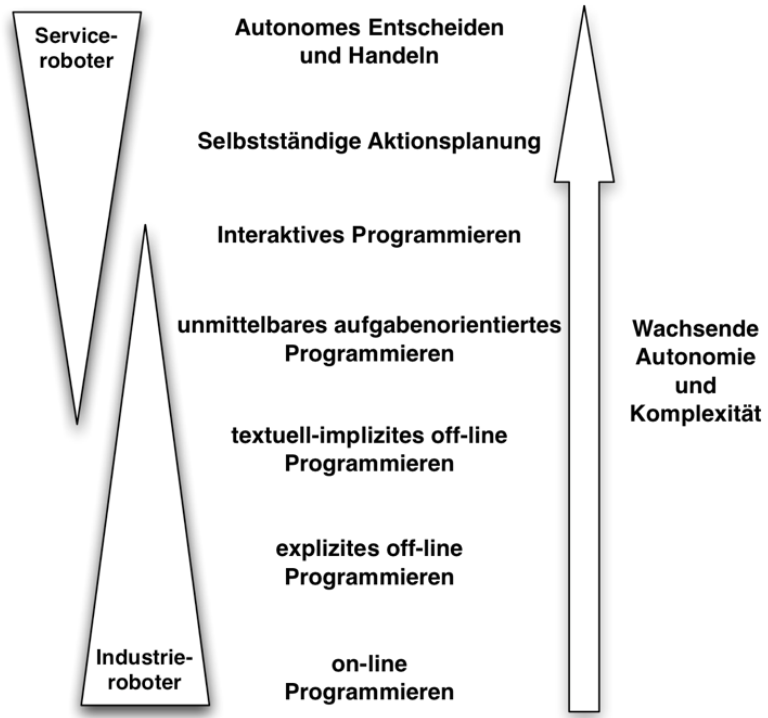
\includegraphics[width=0.5\linewidth]{figures/ch01_ueberblick.png}
\caption{Überblick}
\label{fig:ch01_komp}
\end{figure}
Kriterien:
\begin{itemize}
\item[1.] \textbf{Programmierort:} On-line (prozessnah, am Roboter) vs. Off-line (prozessfern, ohne Roboter)
\item[2.] \textbf{Art der Programmierung:} Direkte vs. indirekte (textuelle oder graphische/gemischte) Programmierung, hybride Verfahren
\item[3.] \textbf{Abstraktionsgrad der Programmierung:} Explizite/bewegungs- bzw. roboterorientierte vs. implizite/aufgabenorientierte Programmierung
\end{itemize}
\begin{figure}[ht]\centering 
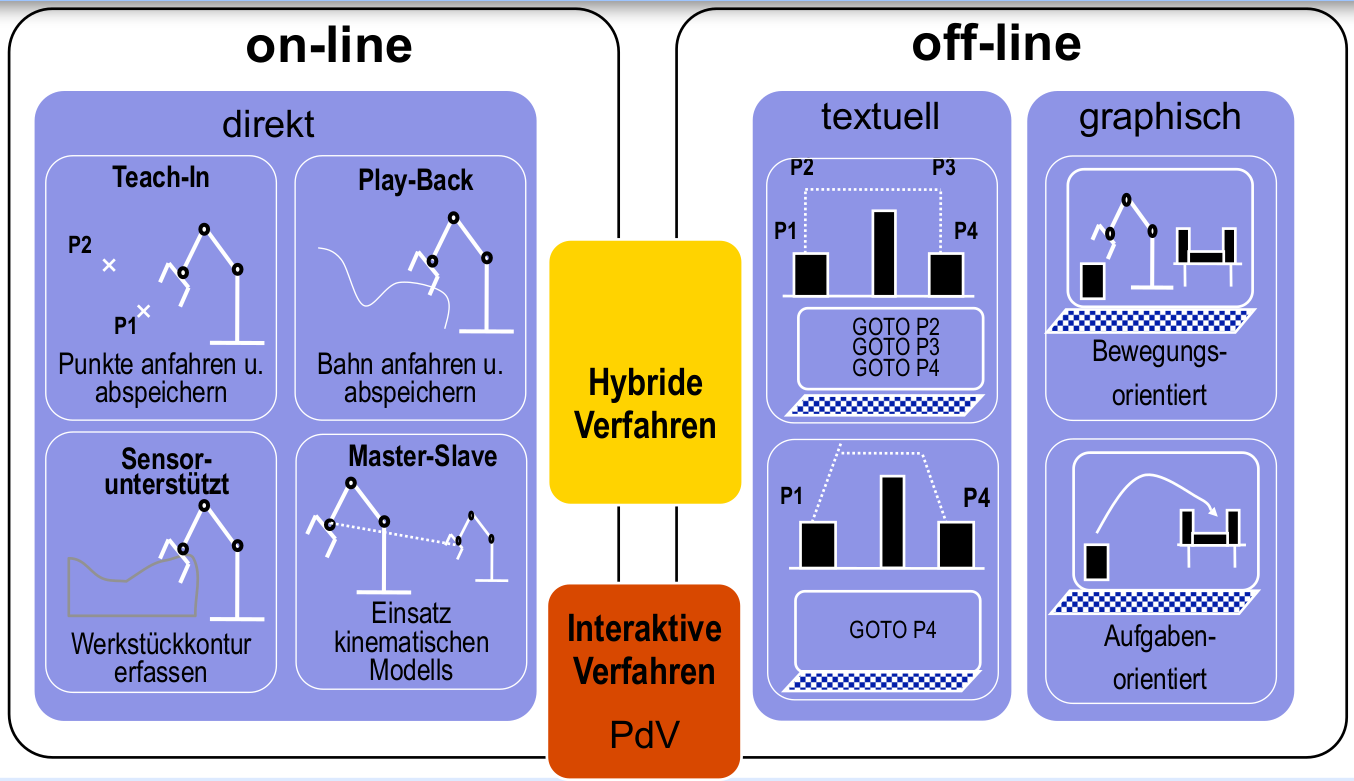
\includegraphics[width=\linewidth]{figures/ch01_schema.png}
\caption{Schema}
\label{fig:ch01_schema}
\end{figure}
\subsection{Arten der Programmierung}
\subsubsection{Direkte/Prozessnahe Programmierung}
\begin{itemize}
\item \textbf{Einstellen des Roboters:} Ältestes Programmierverfahren.
Der Bewegungsbereich jedes Gelenks wird durch Stopper eingeschränkt.
Die Bewegungen erfolgen für jedes Gelenk einzeln bis zum Anschlag.
Zuordnung zwischen Anfahrpunkten zu Stopper kann mit Codiermatritzen erfolgen.
(sogenannter \glqq Bang-Bang-Robot\grqq)\\
Nachteil: sehr kleine Menge von Anfahrpunkten.
\item \textbf{Teach-In Programmierung:} Anfahren markanter Punkte der Bahn mit manueller Steuerung
(Teach Box, Teach Panel, weitere: Spacemouse, Teach-Kugel)\\
Funktionalität einer Teach Box:
\begin{itemize}
\item Einzelbewegung der Gelenke
\item Bewegung des Effektors in 6 Freiheitsgraden
\item Punkte anfahren u. abspeichern
\item Speichern / Löschen von Anfahrpunkten
\item Eingabe von Geschwindigkeiten
\item Eingabe von Befehlen zur Bedienung des Greifers
\item Starten / Stoppen ganzer Programme
\end{itemize}
Vorgehensweise beim Teach-In:
\begin{itemize}
\item Anfahren markanter Punkte der Bahn (= Folge von Zwischenpunkten)
\item Speichern der Gelenkwerte
\item Ergänzung der gespeicherten Werte
um Parameter wie Geschwindigkeit, Beschleunigung usw.
\item Anwendung: in der Fertigungsindustrie (Punktschweißen, Nieten), Handhabungsaufgaben (Pakete vom Fließband nehmen)
\end{itemize}
\item \textbf{Play-Back- (manuelle) Programmierung:}
\begin{itemize}
\item Einstellung des Roboters auf Zero-Force-Control
(Roboter kann durch den Bediener bewegt werden)
\item Abfahren der gewünschten Bahn
\item Speichern der Gelenkwerte: automatisch (definierte Abtastfrequenz) oder manuell (durch Tastendruck)
\item Anwendung: mathematisch schwer beschreibbare Bewegungsabläufe, Integrierung der handwerklichen Erfahrung, typischerweise für Lackieren oder Kleben eingesetzt
\end{itemize}
\begin{table}[hbt]
\centering
\begin{tabular}{|p{13cm}|}
\hline
Nachteile\\
\hline
\vspace{-5mm}
\begin{itemize}
\setlength\itemsep{0em}
\item[-] schwere Roboter schwierig zu bewegen
\item[-] wenig Platz in engen Fertigungszellen für Bediener, dadurch Sicherheitsrisiko
\item[-] hoher Speicherbedarf (bei hoher Abtastrate)
\item[-] schlechte Korrekturmöglichkeiten
\end{itemize}\\
\hline
\end{tabular}
\caption{Nachteile der Play-Back-Programmierung}
\label{tab:PBprog}
\end{table}
\newpage
\item \textbf{Master-Slave-Programmierung:}
\begin{itemize}
\item Bediener führt einen kleinen, leicht bewegbaren Master
Roboter (entspricht einem kinematischen Modell des
Slave-Roboters)
\item Bewegung wird auf den Slave-Roboter übertragen
\item Bewegungen werden synchron ausgeführt
\item Slave-Roboter wirkt als Kraftverstärker
\item Anwendung: Handhabung großer Lasten bzw. großer Roboter
\end{itemize}
\begin{table}[hbt]
\centering
\begin{tabular}{|p{6.5cm}|p{6.5cm}|}
\hline
Vorteile & Nachteile\\
\hline
\vspace{-5mm}
\begin{itemize}
\setlength\itemsep{0em}
\item[+] Möglichkeit, auch schwerste Roboter zu programmieren
\end{itemize}
 &
 \vspace{-5mm}
\begin{itemize}
\setlength\itemsep{0em}
\item[-] teuer, da zwei Roboter benötigt werden
\end{itemize}\\
\hline
\end{tabular}
\caption{Zusammenfassung Master-Slave-Programmierung}
\label{tab:MSprog}
\end{table}
\item \textbf{Sensorunterstützte Programmierung:}\\
Manuell
\begin{itemize}
\item Bediener führt Programmiergriffel (Leuchtstift, Laserstift) entlang der
abzufahrenden Bahn
\item Erfassung der Bewegung durch externe Sensoren (zB. Kameras,
Laserscanner)
\item Berechnung der inversen Kinematik
\end{itemize}
Automatisch
\begin{itemize}
\item Vorgabe des Start- und Zielpunktes
\item Sensorische Ertastung der Sollkontur (zB. über Kraft-Momenten-Sensor)
\end{itemize}
Anwendung: Abspeichern der Bahn als Folge der Gelenkwinkel
Schleifen, Entgraten von Werkstücken	
\end{itemize}
\begin{table}[hbt]
\centering
\begin{tabular}{|p{7.5cm}|p{7.5cm}|}
\hline
Vorteile & Nachteile\\
\hline
\vspace{-5mm}
\begin{itemize}
\setlength\itemsep{0em}
\item[+] schnell bei einfachen Trajektorien
\item[+] sofort anwendbar
\item[+] geringe Fehleranfälligkeit
\item[+] Bediener benötigt keine Programmierkenntnisse
\item[+] kein Modell der Umwelt erforderlich
\end{itemize}
 &
 \vspace{-5mm}
\begin{itemize}
\setlength\itemsep{0em}
\item[-] hoher Aufwand bei komplexen Trajektorien
\item[-] nur mit und am Roboter möglich
\item[-] spezifisch für einen Robotertyp
\item[-] Verletzungsgefahr durch Roboter
\end{itemize}\\
\hline
\end{tabular}
\caption{Zusammenfassung Direkte Programmierung}
\label{tab:dirprog}
\end{table}
\subsubsection{Textuelle Verfahren}
Erstellung von Robotersteuerprogrammen erfolgt mittels erweiterter,
höherer Programmiersprachen (PasRo, Val, etc.)
\\ \\
\textbf{Sprache:} (DIN 66025)
\begin{itemize}
\item Programm = Menge numerierter Sätze\\
z.B. \glqq N70 G00 X20 Z12\grqq{} entspricht Werkzeug im Eilgang (G00) an Position X=20 Z=12 bewegen. (N = Satznummer)
\item Sprachen:
\begin{itemize}
\item APT (Automatically Programmed Tools), 1961 MIT
\item EXAPT (Extended Subset of APT), 1966 Aachen
\end{itemize}
\end{itemize}

\begin{table}[!h]
\centering
\begin{tabular}{|p{7.5cm}|p{7.5cm}|}
\hline
Vorteile & Nachteile\\
\hline
\vspace{-5mm}
\begin{itemize}
\setlength\itemsep{0em}
\item[+] Programmierung kann unabhängig vom Roboter erfolgen
\item[+] strukturierte, übersichtliche Programmierlogik
\item[+] Erstellung komplexer Programme (Einbezug von Wissensbasis,
Weltmodell, Auswertung von Sensoren)
\end{itemize}
 &
 \vspace{-5mm}
\begin{itemize}
\setlength\itemsep{0em}
\item[-] Bediener benötigt Programmierkenntnisse
\item[-] keine / schlechte Korrekturmöglichkeiten
\end{itemize}\\
\hline
\end{tabular}
\caption{Zusammenfassung Textuelle Verfahren}
\label{tab:textprog}
\end{table}
\subsubsection{Graphische/Gemischte Verfahren}
\begin{itemize}
\item Graphische Darstellung von Kontrollstrukturen (if/else, Schleifen,
Marken...)
\item Kopplung mit Visualisierungs-Tool und Simulations-Tool (z.B. RobCAD)
\item  Trajektorien durch Interpolation aus Stützpunkten, Freihandzeichnen,
analytisch
\item Operationen Icon- oder Menu-gesteuert
\item Simple graphische Programmierung, z.B. Lego Mindstorms:
Leicht verständliche, ikonische Programmierung aber beschränkte Möglichkeiten
\item Graphische Programmierung basierend auf sensorieller Erfassung der
Benutzervorführung:\\ Simulation der Roboterprogramme
\end{itemize}
\begin{table}[hbt]
\centering
\begin{tabular}{|p{7.5cm}|p{7.5cm}|}
\hline
Vorteile & Nachteile\\
\hline
\vspace{-5mm}
\begin{itemize}
\setlength\itemsep{0em}
\item[+] Programmierer benötigt weniger Programmierkenntnisse
\item[+] einfache Programmierung, leichte Fehlererkennung
\item[+] schnelles Erstellen komplexer Programme (rapid prototyping)
\end{itemize}
 &
 \vspace{-5mm}
\begin{itemize}
\setlength\itemsep{0em}
\item[-] sensorielle Benutzererfassung noch zu ungenau
\item[-] Leistungsfähige Hardware für Signalanalyse, Modellierung, ...
\item[-] Komplexe Modelle benötigt
\item[-] 2D-Sicht des Anwenders
\end{itemize}\\
\hline
\end{tabular}
\caption{Zusammenfassung Graphische Verfahren}
\label{tab:textprog}
\end{table}
\newpage
\subsection{Abstraktionsgrad der Programmierung}
\subsubsection{Explizite/Roboterorientierte Programmierung}
\textcolor{red}{\glqq Wie ist es zu tun?\grqq} \\
Bewegungen und Greiferbefehle sind direkt in eine Programmiersprache eingebunden.\\
Das Aufgabenmodell ist gegeben durch Anfangs- und Endzustand (z.B. Relationale Darstellung). Ein Beispiel ist in \autoref{cranfield} dargestellt.\\
\begin{figure}[h!]\centering 
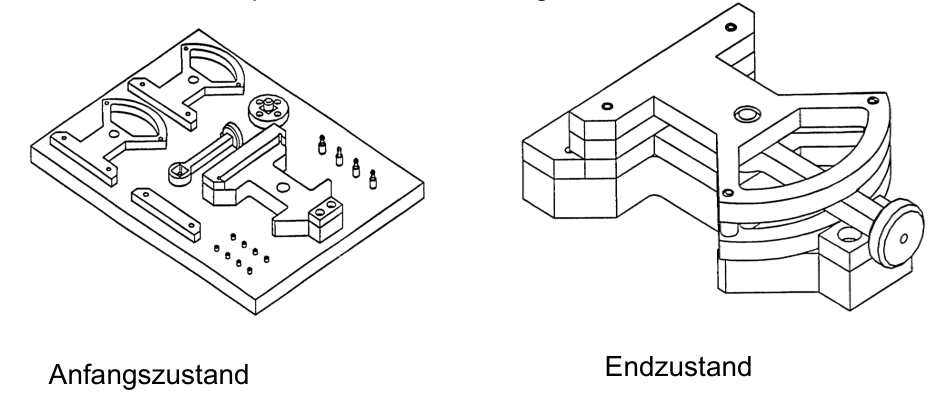
\includegraphics[width=0.7\linewidth]{figures/ch01_cranfield.png}
\caption{Der Cranfield-Montage-Benchmark}
\label{cranfield}
\end{figure}\\
\paragraph{Anwender $\rightarrow$ Roboter}
Jedes Robotersystem besitzt eine roboterabhängige Steuerungsebene, welche folgende Eigenschaften kapselt:
\begin{itemize}
\item Ansteuerung der Hardware (sowohl interne als auch externe)
\item Bewegungsaktionen
\item Lokale Modelle
\item Elementare Operationen (erfordern evtl. Echtzeitregelung)
\end{itemize}
\begin{figure}[h!]\centering 
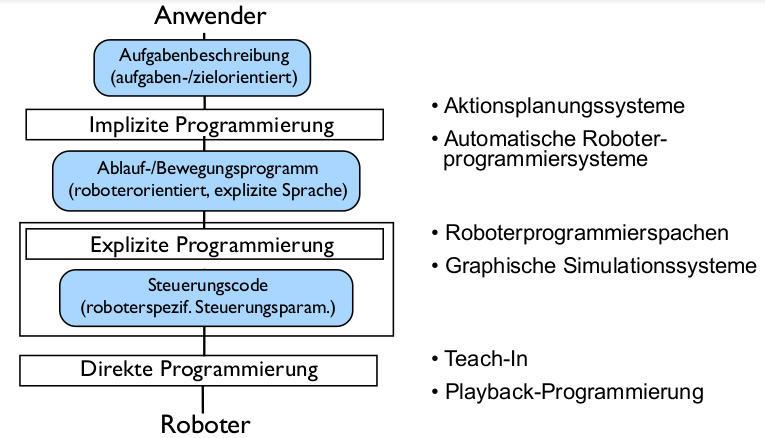
\includegraphics[width=0.7\linewidth]{figures/ch01_einordnung.png}
\caption{Einordnung roboterorientierte Programmierung}
\label{einord}
\end{figure}
\paragraph{Anforderungen an die roboterorientierte Programmierung}
\begin{itemize}
\item Positions-, Geschwindigkeitsregelung der aktiven Komponenten (z.B. Gelenke, Räder)
\item Auslesen und Parametrieren der internen und externen Sensorik
\item Koordinatentransformationen, direkte und inverse Kinematik
\item Sensorabhängige Regelung
\item Verfahren auf Trajektorien
\item Generierung und Zusammensetzen von Trajektorien zu komplexen Bewegungen
\item Verkettung komplexer Bewegungen zu Elementaroperationen
\end{itemize}
\paragraph{Komponenten der roboterorientierten Programmierung}
\autoref{zykl}\\
\begin{figure}[h!]\centering 
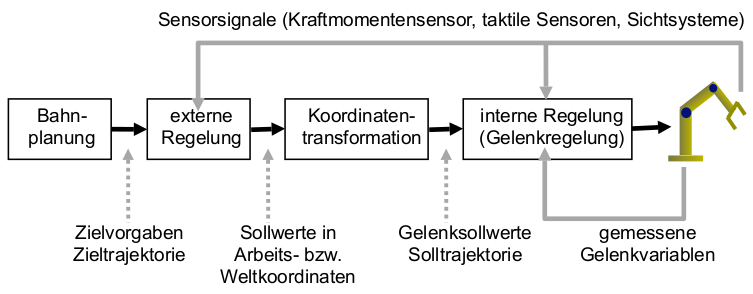
\includegraphics[width=0.7\linewidth]{figures/ch01_zykl.png}
\caption{Regelungszyklus eines Roboters}
\label{zykl}
\end{figure}\\
\paragraph{Sprachelemente von Roboterprogrammiersprachen}
\begin{itemize}
\item Befehle für:
\begin{itemize}
\item Bewegung eines oder mehrerer Roboter
\item Betrieb von Greifern / Werkzeugen
\item Ein-/Ausgabe von Daten / Signalen über Schnittstellen
\item Externe Sensoren
\item Zur Synchronisation / Kommunikation zwischen Prozessen
\item Parallelverarbeitung
\item Zur logischen Verkettung von Koordinatensystemen
\end{itemize}
\item Anweisungen zur Ablaufsteuerung
\item Definition generischer Operationen (zB. Armbewegung + Griff $\rightarrow$ ein Operator)
\end{itemize}
\paragraph{Bewegungsanweisungen}
\begin{itemize}
\item Bewegungen im Gelenkwinkelraum:
\begin{itemize}
\item Bewege alle Gelenke mit max. Geschwindigkeit
\item Regelung der Geschwindigkeiten mit gleichzeitiger Beendigung der Bewegung aller Gelenke
\end{itemize}
\item Kartesische Bewegungen (Stellung des TCPs)
\begin{itemize}
\item Erfordert inverse Kinematik
\item Nutzung von Frames, z.B. relativ zu einem Objekt
\end{itemize}
\item Geometriebezogene Bahndefinition
\end{itemize}
\begin{table}[hbt]
\centering
\begin{tabular}{|p{7.5cm}|p{7.5cm}|}
\hline
Vorteile & Nachteile\\
\hline
\vspace{-5mm}
\begin{itemize}
\setlength\itemsep{0em}
\item[+] Hohe Einstellgenauigkeit der Position
\item[+] Hohe Wiederholgenauigkeit
\item[+] eindeutige Roboterkonfiguration
\item[+] keine inverse Kinematik erforderlich
\end{itemize}
 &
 \vspace{-5mm}
\begin{itemize}
\setlength\itemsep{0em}
\item[-] Abhängigkeit von Robotertyp
\item[-] kein Bezug der Gelenkwinkel zur Objektlage
\end{itemize}\\
\hline
\end{tabular}
\caption{Bewegungen im Gelenkwinkelraum}
\label{tab:bew}
\end{table}
\paragraph{Sprachelemente -- Semantik von Greiferbefehlen}
\begin{itemize}
\item Verschiedene Greifertypen: evtl. mit taktiler und/oder Kraftsensorik
\item Backengreifer: Industrie, Forschung (z.B. 3-Finger-Hand)
\end{itemize}
Mit zunehmender Abstraktion:
\begin{enumerate}
\item Steuerung im Gelenkwinkel-Raum
\begin{itemize}
\item Anzahl der Freiheitsgrade bestimmt Anzahl der Parameter (Backengreifer: 1, menschl. Hand: 22)
\item Wenig Kapselungs-Aufwand (keine inverse Kinematik nötig) 
\item Hand-abhängig
\item Kein Bezug zwischen Fingerstellung und Handstellung
\end{itemize}
\item Steuerung im kartesischen/ zylindrischen/... Raum
\begin{itemize}
\item Parameter: Position/Orientierung jedes Fingers/ jeder Fingerspitze
\item Inverse Kinematik nötig
\item Berechnung aus Greif-/ Bewegungsplanung oder aus menschlicher Vorführung
\item Mögliche Konfigurationen (Konfigurationsraum) handabhängig
\end{itemize}
\item Semantische Steuerung
\begin{itemize}
\item Parameter: Griff-Form, zu greifendes Objekt, Objektgröße, Objektform, ...
\item Mapping auf Roboterhand nötig
\item Übertragbar auf andere Roboterhände (mögliche Griffe handabhängig)
\item Griff-Form vom Menschen lernbar
\end{itemize}
\end{enumerate}
\paragraph{Zusammenfassung -- Explizite Programmierung} Nur in Verbindung mit (abstrakten) Programmiersprachen
\begin{table}[hbt]
\centering
\begin{tabular}{|p{7.5cm}|p{7.5cm}|}
\hline
Vorteile & Nachteile\\
\hline
\vspace{-5mm}
\begin{itemize}
\setlength\itemsep{0em}
\item[+] beliebig komplexe Bahnen
\item[+] Anbindung von Sensoren
\item[+] reaktive Planung
\end{itemize}
 &
 \vspace{-5mm}
\begin{itemize}
\setlength\itemsep{0em}
\item[-] Keine standardisierte Programmiersprache
\item[-] Kenntnis der Programmiersprache
\end{itemize}\\
\hline
\end{tabular}
\caption{Bewegungen im Gelenkwinkelraum}
\label{tab:bew}
\end{table}
\subsubsection{Implizite/Aufgabenorientierte Programmierung}
\textcolor{red}{\glqq Was ist zu tun?\grqq} \\
Die Aufgabe, die der Roboter durchführen soll, wird beschrieben, z.B. in Form von Zuständen.
\begin{itemize}
\item Abstrakte Form der Programmierung erfolgt in den Phasen\\
1. Modellierung der Umwelt\\
2. Spezifikation der Aufgaben\\
3. Erzeugung der Roboterprogramme
\item u. U. erfolgt vor der Ausführung eine Überprüfung des
Roboterprogramms (Simulation)
\item Beispiel: Einschenken unter Berücksichtigung von Hindernissen
\item Details im kommenden Kapitel
\end{itemize}

\section{Aufgabenorientierte Programmierung} %(2. VL)
\subsection{Umweltmodellierung}
\begin{figure}[ht]\centering 
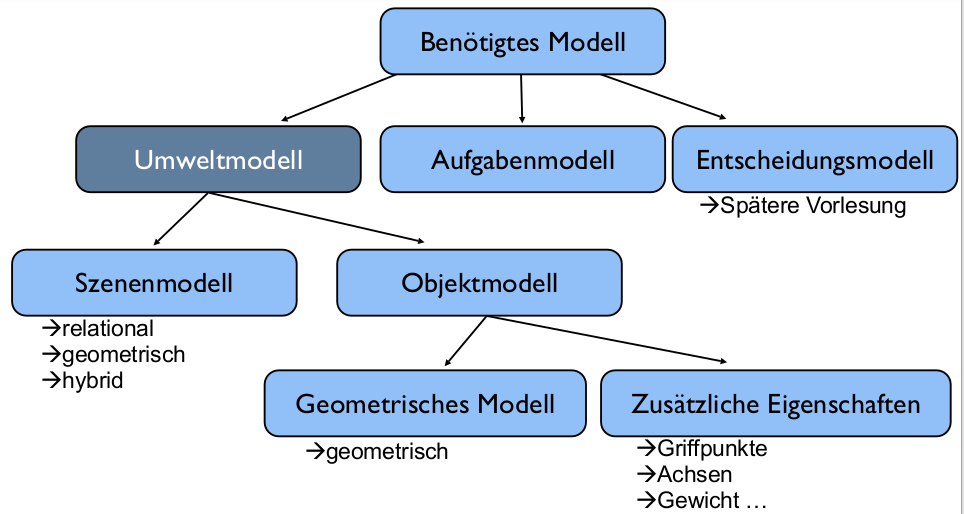
\includegraphics[width=0.6\linewidth]{figures/ch02_umweltmodell.png}
\caption{Umweltmodell}
\label{fig:ch02_um}
\end{figure}

%Keine Umlaute in labels!!!
\subsubsection{Objektmodell}
Die geometrische Beschreibung von Objekten beinhaltet:
\begin{itemize}
\setlength\itemsep{0em}
\item graphische Darstellung
\item Kollisionsberechnungen, Kontaktberechnung in Griffplanung, ...
\item physikalisch-dynamische Simulation der Effekte von Handlungen auf die Umwelt
\item geometriebezogene Bewegungsplanung
\end{itemize}
Es gibt drei Ansätze zur geometrischen Modellierung (\autoref{fig:obrepr}): 
\begin{enumerate}
\item Kantenmodelle
\item Flächenmodelle
\item Volumenmodelle
\end{enumerate}
\begin{figure}[h!]
	\centering
	\begin{subfigure}{.25\textwidth}
		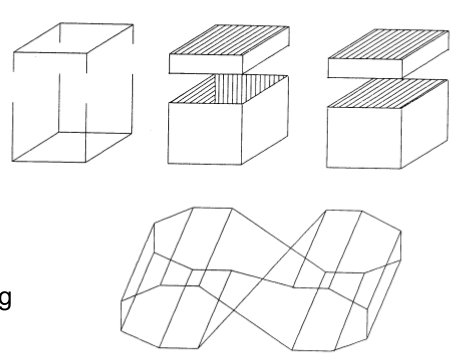
\includegraphics[width=\textwidth]{figures/ch02_kanten.png}
		\caption{}
	\end{subfigure}
	\begin{subfigure}{.25\textwidth}
		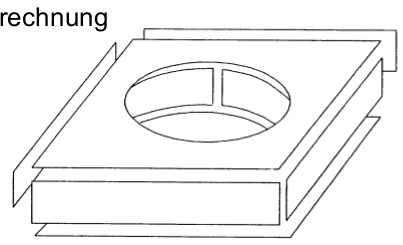
\includegraphics[width=\textwidth]{figures/ch02_flaechen.png}
		\caption{}
	\end{subfigure}
	\begin{subfigure}{.25\textwidth}
		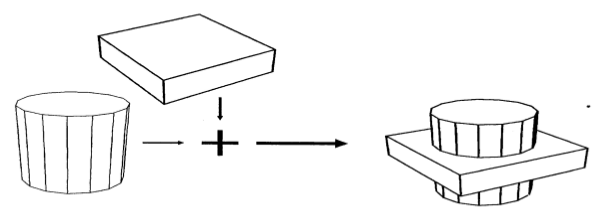
\includegraphics[width=\textwidth]{figures/ch02_volumen.png}
		\caption{}
	\end{subfigure}
	\caption{Objektrepr\"{a}entation}
	\label{fig:obrepr}
\end{figure}
\paragraph*{Kanten}
Nur die Kanten werden gespeichert, d.h. Punkte und Verbindungen (Gerade, Polygonzug, Bezierkurve, ... ).
\begin{table}[hbt]
\centering
\begin{tabular}{|p{6.5cm}|p{6.5cm}|}
\hline
Vorteile & Nachteile\\
\hline
\vspace{-5mm}
\begin{itemize}
\setlength\itemsep{0em}
\item[+] einfache Daten
\item[+] wenige Daten
\end{itemize}
 &
 \vspace{-5mm}
\begin{itemize}
\setlength\itemsep{0em}
\item[-] Mehrdeutigkeiten
\item[-] hoher Eingabeaufwand
\item[-] keine Kollisionsberechnung
\item[-] kein Schnitt
\end{itemize}\\
\hline
\end{tabular}
\caption{Zusammenfassung -- Kantenmodelle}
\label{tab:Kantenmod}
\end{table}\\ 
\paragraph*{Flächen}
Flächen können exakt modelliert werden, wenn sie \textcolor{red}{analytisch gegeben} sind (eine 3D Kugel beispielsweise durch $r = ||x-p||$, wobei $r$ der Radius und $p$ der Mittelpunkt ist).
\begin{table}[hbt]
\centering
\begin{tabular}{|p{6.5cm}|p{6.5cm}|}
\hline
Vorteile & Nachteile\\
\hline
\vspace{-5mm}
\begin{itemize}
\setlength\itemsep{0em}
\item[+] Geschlossene Darstellung (wenig Speicherbedarf)
\item[+] Analytische Darstellung erlaubt einfache Rechenverfahren (z.B.
Schnitt von Ebenen / Kugeln $\rightarrow$ schnelle Kollisionsberechnung)
\end{itemize}
 &
 \vspace{-5mm}
\begin{itemize}
\setlength\itemsep{0em}
\item[-] Wenige Flächen sind analytisch darstellbar
\end{itemize}\\
\hline
\end{tabular}
\caption{Flächen -- analytisch}
\label{tab:Flaechen-analyt}
\end{table}\\ 
Ansonsten werden sie \textcolor{red}{approximativ} durch Bildung einer großen Fläche aus einem Netz (\glqq Mesh\grqq ) von einfachen Einzelflächen (z.B. Dreiecke, Vierecke) modelliert.\\
\begin{table}[hbt]
\centering
\begin{tabular}{|p{6.5cm}|p{6.5cm}|}
\hline
Vorteile & Nachteile\\
\hline
\vspace{-5mm}
\begin{itemize}
\setlength\itemsep{0em}
\item[+] Definition sehr einfach
\item[+] einfache Algorithmen
\end{itemize}
 &
 \vspace{-5mm}
\begin{itemize}
\setlength\itemsep{0em}
\item[-] hoher Speicherbedarf
\item[-] hoher Rechenaufwand
\end{itemize}\\
\hline
\end{tabular}
\caption{Flächen -- approximativ}
\label{tab:Flaechen_approx}
\end{table}
\newpage
Hierbei werden Freiformflächen im einfachsten Fall durch \textbf{Dreiecksflächen} approximiert:
\begin{itemize}
\item[] Gegeben seien 3 Punkte im Raum $P_1 , P_2 , P_3$.
\item[] Damit hat die Fläche folgende Gleichung: $F(u,v)=u\cdot P_1 +v\cdot P_2 +(1-u-v)\cdot P_3$ mit $0 \leq u,v, u+v \leq 1$.
\begin{center}
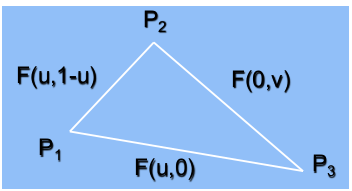
\includegraphics[width=.3\linewidth]{figures/ch02_dreieck.png}
\end{center}
\end{itemize}
Oder sie werden durch \textbf{Bilineare Viereckselemente / Pflaster} approximiert:
\begin{itemize}
\item[] Gegeben sind 4 Punkte im Raum $P_1 , P_2 , P_3, P_4$
\item[] Damit wird die Fläche definiert durch $F(u,v)=(1-u)(1-v) \cdot P_1 + (1-u)v \cdot P_2 + u(1-v) \cdot P_3 + uv \cdot P_4$ mit $0 \leq u \leq 1, 0 \leq v \leq 1$. 
\begin{center}
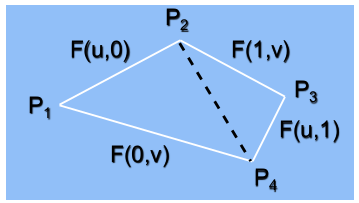
\includegraphics[width=.3\linewidth]{figures/ch02_pflaster.png}
\end{center}
\end{itemize}
\begin{table}[hbt]
\centering
\begin{tabular}{|p{6.5cm}|p{6.5cm}|}
\hline
Vorteile & Nachteile\\
\hline
\vspace{-5mm}
\begin{itemize}
\setlength\itemsep{0em}
\item[+] Flächenelemente können gekrümmt sein
$\rightarrow$ weniger Gitterpunkte bei gleich guter Approximation
\end{itemize}
 &
 \vspace{-5mm}
\begin{itemize}
\setlength\itemsep{0em}
\item[-] Rechnen mit gekrümmten Flächen ist aufwendig
\end{itemize}\\
\hline
\end{tabular}
\caption{Approximation durch Vierecke}
\label{tab:Viereck_approx}
\end{table}
Zudem können Flächen durch \textbf{Bezierflächen}, einer Erweiterung der Bezierkurven beschrieben werden:
\begin{itemize}
\item[] Gegeben ist ein Gitter von Führungspunkten $P_{ij}, 0 \leq i \leq N$ und $0 \leq j \leq M$.
\item[] Damit ist die Fläche beschrieben durch $F(u,v) = \sum_{i=0}^N \sum_{j=0}^M P_{ij} \cdot B_{i,N}(u) \cdot B_{j,M}(v)$\\
 mit $B_{i,N}(u) = (1-u)B_{i,N-1}(u)+uB_{i-1,N-1}(u)$\\
 und $B_{j,M}(v) = (1-v)B_{j,M-1}(v)+vB_{j-1,M-1}(v)$.
\item[] Die $B_{i,N}$ bzw. $B_{j,M}$ heißen auch Bernsteinpolynome.
\begin{center}
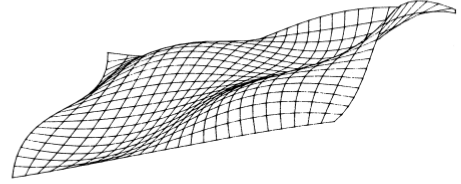
\includegraphics[width=.4\linewidth]{figures/ch02_bezier.png}
\end{center}
\end{itemize}
\begin{table}[hbt]
\centering
\begin{tabular}{|p{6.5cm}|p{6.5cm}|}
\hline
Vorteile & Nachteile\\
\hline
\vspace{-5mm}
\begin{itemize}
\setlength\itemsep{0em}
\item[+] effiziente Verfahren 
\item[+] entspricht dem Vorgehen während der Modellierung
\item[+] schnelle Kollisions- und Abstandsberechnung
\end{itemize}
 &
 \vspace{-5mm}
\begin{itemize}
\setlength\itemsep{0em}
\item[-] hoher Eingabeaufwand
\item[-] Darstellung aufwendig
\item[-] Problem bei Schnittoperationen
\item[-] Inkonsistenzen möglich
\end{itemize}\\
\hline
\end{tabular}
\caption{Zusammenfassung -- Flächenmodelle}
\label{tab:Flaechenmod}
\end{table}
\noindent
\paragraph*{Volumen} Vier verschiedene Arten von Volumenmodellen:\\ \\
\textbf{Parametrische Modelle}:\\
Grundkörper und topologische Operationen auf diesen (Schnitt, Vereinigung, ... ) werden abgespeichert. 
\begin{table}[hbt]
\centering
\begin{tabular}{|p{6.5cm}|p{6.5cm}|}
\hline
Vorteile & Nachteile\\
\hline
\vspace{-5mm}
\begin{itemize}
\setlength\itemsep{0em}
\item[+] eindeutige Objektbeschreibung 
\item[+] geringer Eingabeaufwand 
\item[+] Ergebnis von Operationen sind korrekte Objekte
\end{itemize}
 &
 \vspace{-5mm}
\begin{itemize}
\setlength\itemsep{0em}
\item[-] hoher Implementierungsaufwand
\item[-] Einbindung von Freiformflächen schwierig
\end{itemize}\\
\hline
\end{tabular}
\caption{Volumenmodelle -- parametrisch}
\label{tab:Volmod}
\end{table}\\ 
Die Objekte sind bereits vorhanden und können durch Angabe von Parametern angepaßt werden (Varianten).\\
Konsistenzprüfungen sind notwendig (\autoref{fig:kons})! \\
\begin{figure}[h!]
	\centering 
	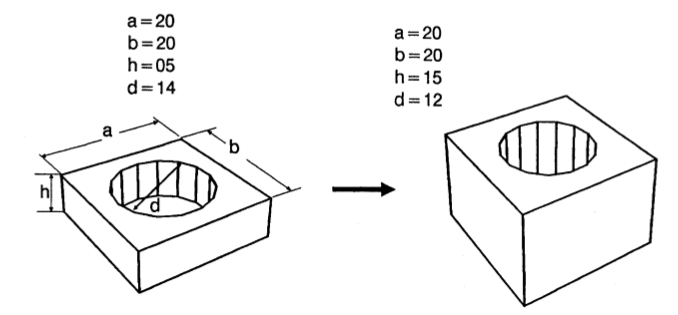
\includegraphics[width=0.3\linewidth]{figures/ch02_kons.png}
	\caption{Konsistenzprüfung: $d < min(a,b)$}
\label{fig:kons}
\end{figure}\\
\noindent
\textbf{Zellenzerlegung}:\\
 Objekte werden aus disjunkten Elementarzellen aufgebaut. Verwendung finden einfache geometrische Objekte z,B. Tetraeder, Quader, ...
Benutzt in der Strukturanalyse mit Finite-Elemente-Methoden (FEM).
\newpage
Diese Modelle können auf drei Arten umgesetzt werden:
\begin{enumerate}
\item Boundary Repräsentation
\item Constructive Solid Geometry (CSG)
\item Zellenbelegung
\end{enumerate}
\textbf{Boundary Repräsentation}: Hierarchische Darstellung eines Objektes durch begrenzende
Elemente, i.d.R. Kanten oder Flächen. \autoref{fig:brep} zeigt ein Beispiel.\\
\begin{figure}[h!]
	\centering 
	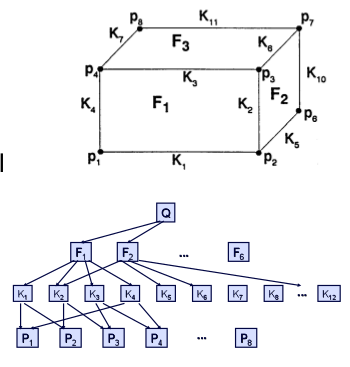
\includegraphics[width=0.3\linewidth]{figures/ch02_brep.png}
	\caption{Elemente eines Quaders im Flächenmodell: Quader $Q$, Flächen $F_i : i \in \{1,...,6\}$, Kanten $K_i : i \in \{1,...,12\}$, Ecken $P_i : i \in \{1,...,8\}$}
\label{fig:brep}
\end{figure}
Vorteile: aus der topologischen Struktur Information über z.B.:
\begin{itemize}
\item Welche Flächen gehören zum Objekt?
\item Welche Kanten gehören zur Fläche? $\rightarrow$ kantenbasierte Objekterkennung
\item Zu welchem Objekt gehört eine Fläche?
\item Zu welchem Objekt gehört eine Kante?
\item Welche Flächen stoßen aneinander?
\end{itemize}
\noindent
\textbf{Constructive Solid Geometry (CSG)}:
Es gibt eine Menge von einfachen Grundkörpern, die parametriert
werden können (\autoref{fig:csg}). 
\begin{figure}[h!]
	\centering
	\begin{subfigure}{.7\textwidth}
		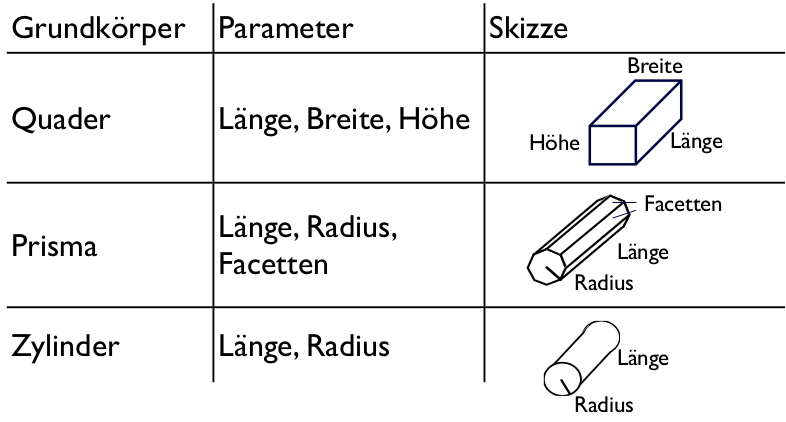
\includegraphics[width=\textwidth]{figures/ch02_csg.png}
	\end{subfigure}
	\begin{subfigure}{.7\textwidth}
		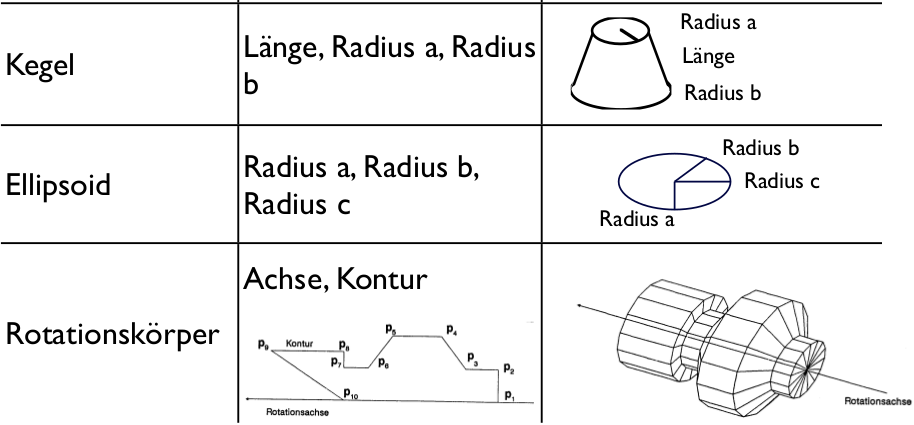
\includegraphics[width=\textwidth]{figures/ch02_csg1.png}
	\end{subfigure}
	\caption{Constructive Solid Geometry}
	\label{fig:csg}
\end{figure}
Auf ihnen sind verschiedene Operationen definiert, z.B.
\begin{table}[!hb]
\centering
\begin{tabular}{|p{6.5cm}|p{6.5cm}|}
\hline
Objekt $A$ 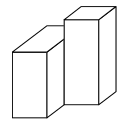
\includegraphics[width=.07\textwidth]{figures/ch02_a.png} & Objekt $B$ 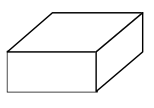
\includegraphics[width=.07\textwidth]{figures/ch02_b.png}\\
\hline
Vereinigung $A \cup B$ (Summe) & 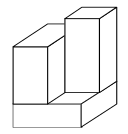
\includegraphics[width=.07\textwidth]{figures/ch02_ab.png}\\
\hline
Schnitt $A \cap B$ & 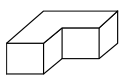
\includegraphics[width=.07\textwidth]{figures/ch02_ab1.png} \\
\hline
Differenz $A / B$ & 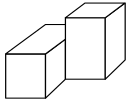
\includegraphics[width=.07\textwidth]{figures/ch02_ab2.png}\\
\hline
Sweep:
Ein Grundelement (u.U. eine Fläche) wird entlang einer Raumkurve
verschoben. Der durchdrungene Raum stellt das neue Objekt dar. & \\
\hline
\end{tabular}
\caption{CSG -- Operatoren}
\label{tab:csg_ops}
\end{table}\\ \\
\textbf{Zellenbelegung}:
Der Raum wird in mehrere Zellen unterteilt (i.d.R. 8 Zellen: \glqq Octree\grqq).
Wenn eine Zelle komplett vom Objekt belegt ist, als \glqq belegt\grqq{} markieren.
Wenn die Zelle nur teilweise belegt ist, dann wird auf diese Zelle das
Verfahren rekursiv angewendet. Ansonsten ist die Zelle leer.
Die Rekursion terminiert bei einer vorbestimmten minimalen Zellgröße.
Teilbelegte kleinste Zellen werden als belegt markiert. Siehe \autoref{zb}.
\begin{figure}[h!]
	\centering
	\begin{subfigure}{.45\textwidth}
		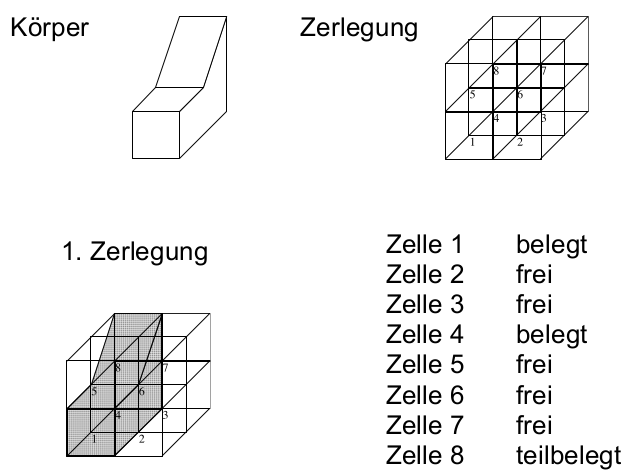
\includegraphics[width=\textwidth]{figures/ch02_zb.png}
	\end{subfigure}
	\begin{subfigure}{.45\textwidth}
		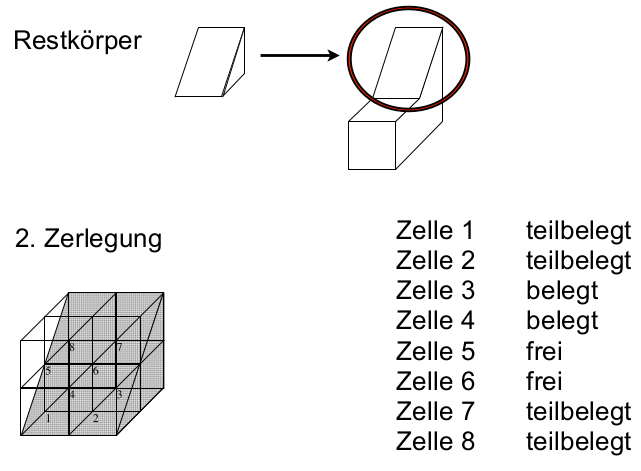
\includegraphics[width=\textwidth]{figures/ch02_zb1.png}
	\end{subfigure}
	\caption{Beispiel -- Zellenbelegung}
	\label{zb}
\end{figure}
\newpage
\subsection{Aufgabenmodellierung}
\begin{figure}[h!]\centering 
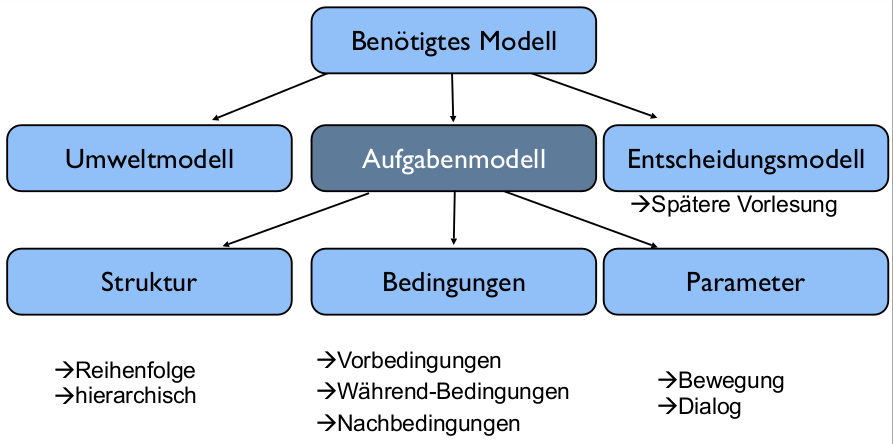
\includegraphics[width=0.6\linewidth]{figures/ch02_aufgabenmodell.png}
\caption{Aufgabenmodell}
\label{fig:ch02_am}
\end{figure}
%kognitive Lücke?
\begin{figure}[ht]\centering 
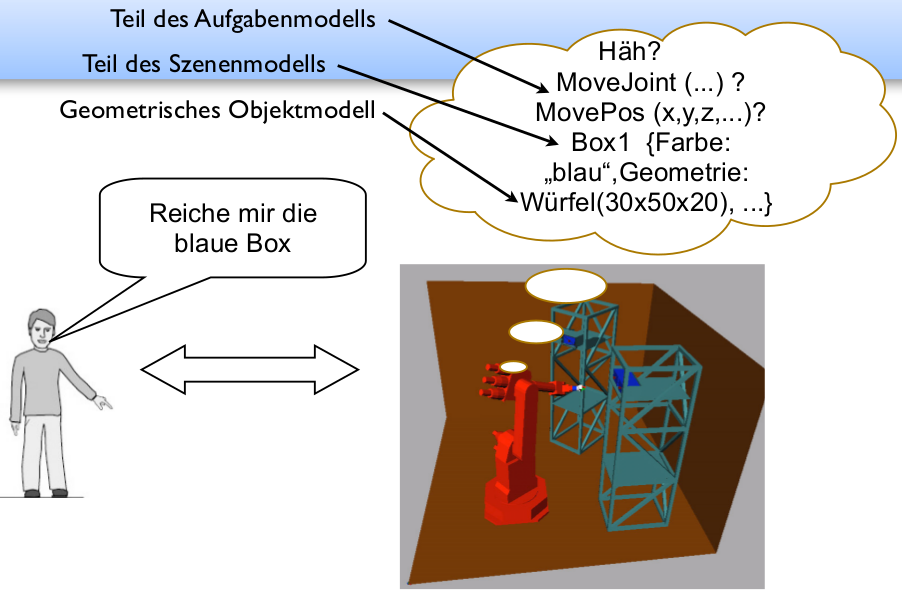
\includegraphics[width=0.6\linewidth]{figures/ch02_beispiel.png}
\caption{Beispiel}
\label{fig:ch02_bsp}
\end{figure}
\begin{figure}[h!]\centering 
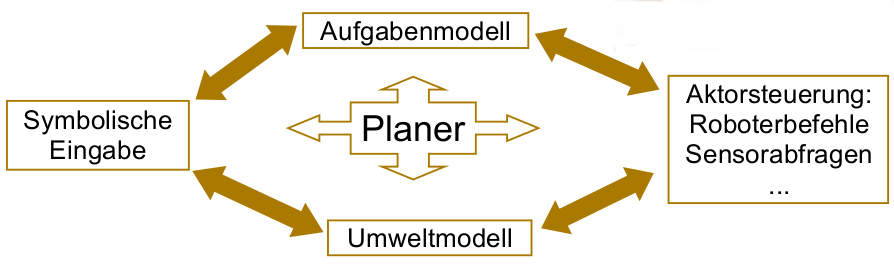
\includegraphics[width=0.6\linewidth]{figures/ch02_planer.png}
\caption{Einordnung des Aufgabenmodells}
\label{fig:ch02_ord}
\end{figure}
\textbf{Anforderungen an das Aufgabenmodell}:
\begin{itemize}
\item Erweiterbarkeit
\item Erklärbarkeit
\item Wiederverwendbarkeit
\item Integration des Wissens in ein Planungssystem
\end{itemize}
\newpage
\paragraph*{Symbolische Abstraktion}
Benutzer beschreibt die Aufgabe mit seinen Worten\\ (z.B. \glqq Bring mir Tee!\grqq) 
\begin{itemize}
\ita Abbildung: Erzeugung der Roboterbefehle über mehrere Stufen (vgl. \autoref{symbab})
\ita \glqq Fahre in die ‚Küche‘, greife ein Glas, fahre zurück und reiche mir den Becher.\grqq
\ita \glqq DriveTo(...), SearchObject(...), MoveArm(...), Grasp(Becher), MoveArm(...), DriveTo(...), MoveArm(...) ...!\grqq
\end{itemize}
\begin{figure}[h!]\centering 
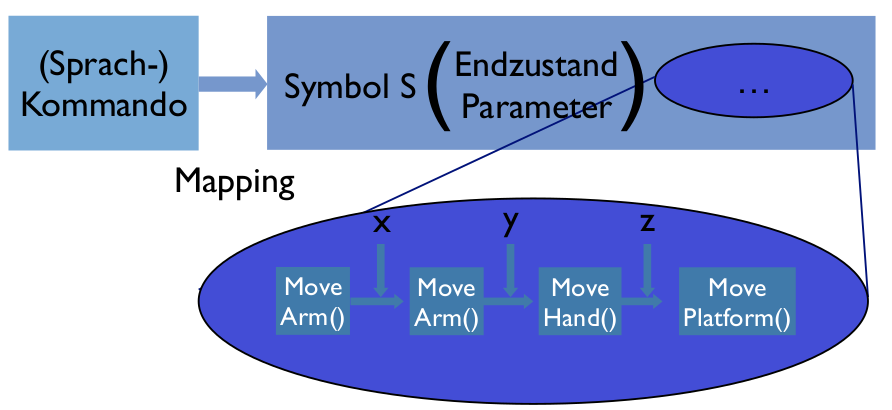
\includegraphics[width=0.6\linewidth]{figures/ch02_symbab.png}
\caption{Symbolische Abstraktion}
\label{symbab}
\end{figure}
\paragraph*{Modellierung der Reihenfolge von Operatoren/Symbolische Handlungsatome}
\begin{itemize}
\item In den gegebenen Beispielen wurden bereits implizit Handlungsatome angenommen
\item Die kleinsten auszuführenden Handlungseinheiten werden als
Elementaroperationen oder atomare Handlungen bezeichnet.
\item Komplexe Handlungen werden aus Elementaroperationen zusammengesetzt. Diese
können dazu üblicherweise parametriert werden.
\item Jeder Roboter besitzt eine endliche Menge an Elementaroperationen.
\end{itemize}
\paragraph*{Drei Ansätze für das Aufgabenmodell}
\begin{enumerate}
\item Sequentiell (\autoref{seq}): Festgelegte Folge von elementaren Aktionen 
\item Vorranggraph (\autoref{vorgra}): Darstellung der Abhängigkeiten
\item Hierarchisch (\autoref{hierar}): Abstraktion von Teilhandlungen
\end{enumerate}
\begin{figure}[h!]
	\centering
	\begin{subfigure}{.25\textwidth}
		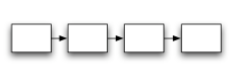
\includegraphics[width=\textwidth]{figures/ch02_ans.png}
		\caption{Sequentiell}
		\label{seq}
	\end{subfigure}
	\begin{subfigure}{.25\textwidth}
		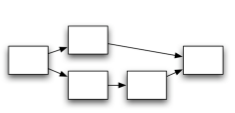
\includegraphics[width=\textwidth]{figures/ch02_ans1.png}
		\caption{Vorranggraph}
		\label{vorgra}
	\end{subfigure}
		\begin{subfigure}{.25\textwidth}
		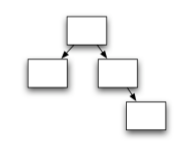
\includegraphics[width=\textwidth]{figures/ch02_ans2.png}
		\caption{Hierarchie}
		\label{hierar}
	\end{subfigure}
	\caption{Ansätze für das Aufgabenmodell}
	\label{ans}
\end{figure}
\newpage
\textbf{Sequentielle Handlungsbeschreibung}:
\begin{itemize}
\item Folge von (parametrierten) atomaren Handlungen
\item Eindeutig festgelegte Reihenfolge
\item Reihenfolge und Anordnung nicht unbedingt erklärbar (lesbar)
\item Bedingungen, Alternativen, etc. schlecht darstellbar
\item Sinnvoll für einfache Aufgaben oder sehr strukturierte Umgebungen (z.B. Leittechnik/Industrie)
\item Komplexe Handlungen: Rein sequentielle Beschreibungen nicht mächtig genug!
\item Ausführung sequentiell beschriebener Handlungen trivial
\item Linearer Handlungsfluss
\item Ausführung besteht aus: Anstoßen einer Elementarhandlung, evtl. Handlungsüberwachung und nach (erfolgreicher) Beendigung Übergang zur nächsten Elementarhandlung
\item Einfache Mechanismen zur Ausführung nötig!
\end{itemize}
\textbf{Vorranggraph}:
\begin{figure}[h!]
	\centering
	\begin{subfigure}{.45\textwidth}
		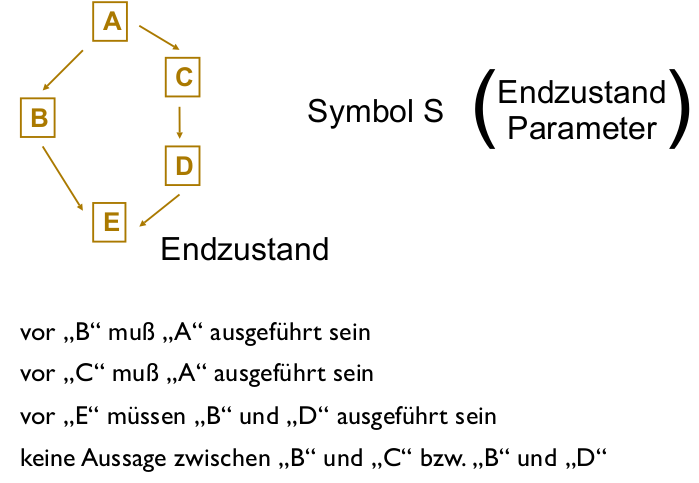
\includegraphics[width=\textwidth]{figures/ch02_vg-mod.png}
		\caption{Modellierung der Reihenfolge: Vorranggraph}
	\end{subfigure}
	\begin{subfigure}{.45\textwidth}
		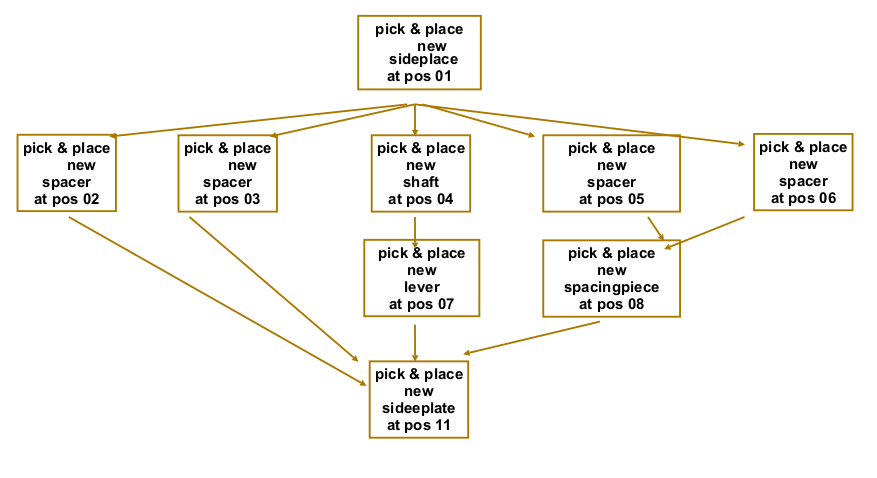
\includegraphics[width=\textwidth]{figures/ch02_vg-bsp.png}
		\caption{Beispiel: Vorranggraph des Cranfield-Benchmarks (simple Montage-Aufgabe)}
		\label{vg}
	\end{subfigure}
	\caption{Vorranggraph}
	\label{vg1}
\end{figure}
\begin{itemize}
\item Darstellung der Handlung in mehreren unabhängigen Teilzweigen
\item Üblicherweise: Serialisierung notwendig!
\begin{itemize}
\item Berechnung optimaler Operatorreihenfolgen
\item Freiheitsgrad zum Ausführungszeitpunkt
\item Serialisierung aufwendig ($\rightarrow$ Planungsverfahren, siehe spätere Vorlesungen)
\end{itemize}
\item Ausführung beinhaltet also:
\begin{itemize}
\item Serialisierung der Handlung nach gegebenen Kriterien
\item Ausführung der sequentiell beschriebenen Handlung
\end{itemize}
\item Mächtigere Handlungsbeschreibung benötigt auch mächtigere Verfahren bei der Ausführung!
\end{itemize}
\textbf{Hierarchisches Aufgabenmodell} (Abbildungen \ref{hier} und \ref{hiermod}):\\
Sowohl Aufgabenspezifikation als auch Aufgabenzerlegung/-teilung sind hierarchisch strukturiert. Die Abstraktion erfolgt nach Raum, Zeit, Objekten und Alternativen.
\begin{figure}[h!]\centering 
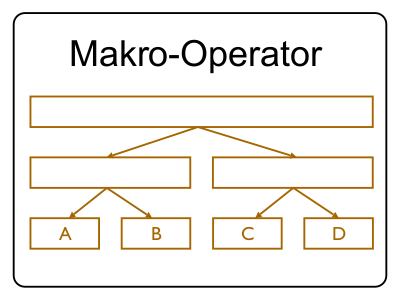
\includegraphics[width=0.3\linewidth]{figures/ch02_hier.png}
\caption{}
\label{hier}
\end{figure}\\
\begin{figure}[h!]
	\centering
	\begin{subfigure}{.45\textwidth}
		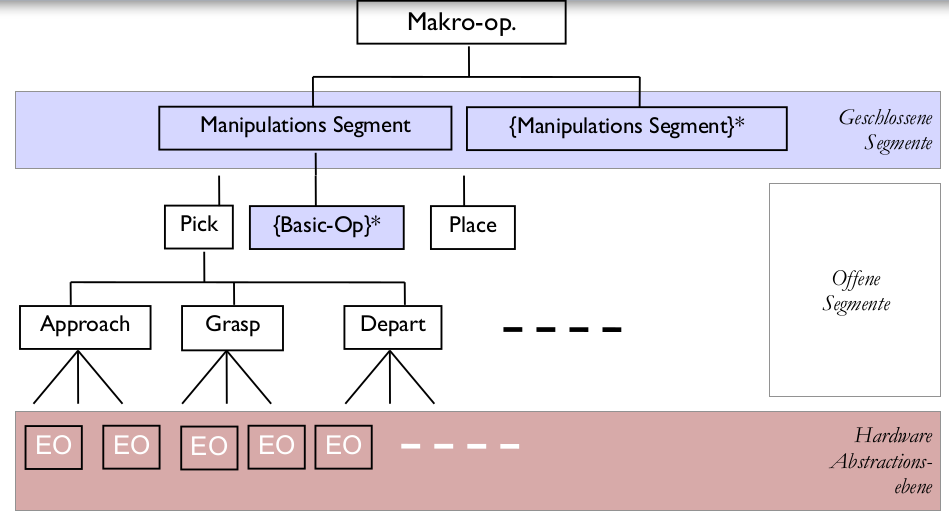
\includegraphics[width=\textwidth]{figures/ch02_hier1.png}
		\caption{Semantische hierarchische Repräsentation}
	\end{subfigure}
	\begin{subfigure}{.45\textwidth}
		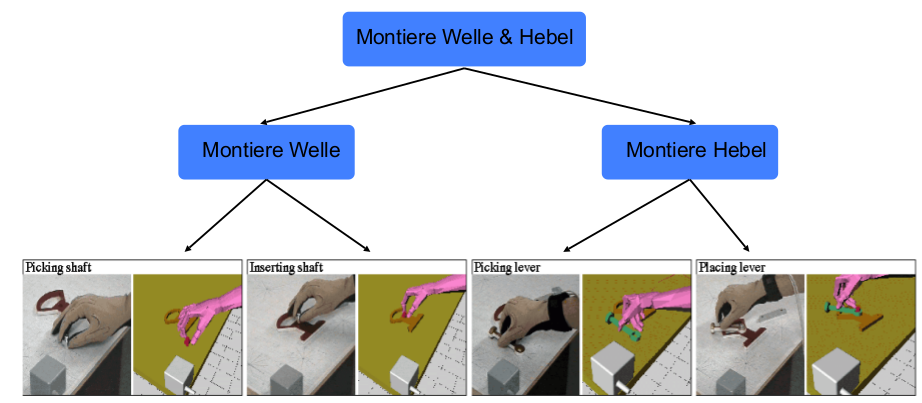
\includegraphics[width=\textwidth]{figures/ch02_hier2.png}
		\caption{Programmbeispiel: Montage von Welle und Hebel des Cranfield Benchmarks}
	\end{subfigure}
	\caption{Hierarchisches Aufgabenmodell}
	\label{hiermod}
\end{figure}
\paragraph*{Abstraktionsebenen im Aufgabenmodell}
Häufige Unterscheidung der in \autoref{abst} dargestellten semantischen Abstraktionsstufen. Diese benutzen symbolische Parameter.
\begin{itemize}
\ita Komplexität der Aufgabe beherrschbar
\ita Formalismen anwendbar
\end{itemize}
\begin{figure}[h!]\centering 
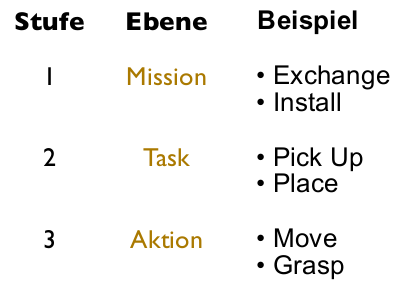
\includegraphics[width=0.3\linewidth]{figures/ch02_abst.png}
\caption{}
\label{abst}
\end{figure}
\textbf{Wahl der Abstraktionsebene}: Wie wird die Abstraktionsebene der Aktion gewählt, damit Aktionen von Roboter A auf Roboter B übertragen werden können?
\begin{itemize}
\item Aktion: Kleinste symbolische Einheit
\item Darunter: Regelungsebene
\item Abhängig von:
\begin{itemize}
\item Komplexität der Aufgabe
\item Grad der Kopplung einzelner Teilhandlungen
\item Hardware: Getrennt geregelte Komponenten werden üblicherweise auch mit getrennten Aktionen modelliert
\item Planungssystem/Beobachtungssystem
\end{itemize}
\item Grundsätzlich: Die Frage ist in der Forschung noch nicht eindeutig geklärt, immer noch ein Streitpunkt!
\end{itemize}
\textbf{Modellierung von Aktionen / Tasks}:\\
Ein \textcolor{red}{Operator} ist definiert durch $OP = (N, O, A, Par, K)$ mit
\begin{itemize}
\item $N$ = Name des Operators (eindeutig)
\item $O$ = Liste der beteiligten Objekte
\item $A$ = Auswahlbedingung
\item $Par$ = Liste der Parameter, z.B. Positionen, Kräfte, Beschleunigungen ...
\item $K$ = Körper des Operators:
\begin{itemize}
\item \textcolor{red}{\textbf{Aktion}/Elementaroperator}:\\ ausführbares Programm\\ $\Rightarrow$ Realisierung einfacher Fähigkeiten
\item \textcolor{red}{\textbf{Task}/Makro-Operator}:\\ besteht aus weiteren Operationen $K = K_1K_2...K_n$ $\Rightarrow$\\ Realisierung einfacher Fähigkeiten
\end{itemize}
\end{itemize}
\textbf{Hierarchische Repräsentation -- Ausführung}:
\begin{itemize}
\item Im Aufgabenmodell ist die Serialisierung implizit gegeben
\begin{itemize}
\item Minimaler Aufwand zur Ausführung
\item Aber: Bei Parallelitäten von Teilhandlungen: Konflikte möglich!
\end{itemize}
\item Ausführung beinhaltet also:
\begin{itemize}
\item Überprüfung auf Konflikte
\item Gegebenenfalls Serialisierung/Lösen der Konflikte
\item Ausführung der resultierenden Operatorsequenz
\end{itemize}
\item Vorteil: Zusammengesetzte (Teil-)Programme können wiederverwendet werden
\item Repräsentation gut \glqq lesbar\grqq{} (verständlich, erklärbar)
\end{itemize}
\textbf{Anwendung hierarchischer Handlungsbeschreibung in der Realität  \\-- Flexible Programme}:\\
Symbolische Abstraktionsebene zur Roboterprogrammierung
\begin{itemize}
\item Hierarchische Handlungsbeschreibung
\item Erklärbar, verständlich, intuitiv
\item Wiederverwendbarkeit
\item Parametrierbar
\item Unterstützt: Bedingungen, Verzweigungen, Ressourcenverwaltung, Parallelität
\item Aufbau flexibler Programme:
\begin{itemize}
\item Repräsentation des Handlungswissens als Baumstruktur
\item Parametrierbare Aktionsbeschreibung
\item Blätter entsprechen Roboteraktionen
\item Abarbeitung entsprechend einer Tiefensuche
\item Instantiierung der Kinder zur Laufzeit (Expansion des Baums)
\item Auswahl des geeignetsten Kandidaten beim expandieren
\item Parallele Ausführung mehrerer Kinder möglich
\end{itemize}
\end{itemize}
\paragraph*{Validierung der Modelle: Simulation oder Graphische Animation}
\begin{enumerate}
\item \textbf{Simulation der Komponenten}: Validierung anhand gegebener Einschränkungen (Kollisionen, Erreichbarkeit, Optimalitätskriterien: Weg, Zeit, Energie, ...)
\begin{itemize}
\ita Für die Simulation von Effekten durch Manipulators wird die Physiksimulation verwendet: Masse, Reibung, Kräfte, Gelenke
\end{itemize}
\item \textbf{Graphische Animation}: Der Anwender überprüft visuell die erstellten Modelle
\begin{itemize}
\ita Wenn die Robotersimulationen ergeben, dass die Zielstellung angefahren werden kann, wird die Bewegung in einer Animation graphisch dargestellt.
\end{itemize}
\end{enumerate}

\paragraph*{Aufgabenmodell -- Zusammenfassung und Diskussion}:\newline
\textbf{Zusammenfassung}:
\begin{itemize}
\item Aufgabenmodell basiert auf elementaren Operationen
\item Oft dreischichtiger Ansatz: Aktion, Task, Mission
\item Verknüpfung der elementaren Operationen zu komplexen Aufgaben:
\begin{itemize}
\item Sequentiell
\item Vorranggraph
\item  Hierarchisch
\item (Kontrollstrukturen)
\end{itemize}
\item Problem: Validierung der Programme
\begin{itemize}
\item Simulation
\item Animation und Validierung durch den Menschen
\end{itemize}
\end{itemize}

\textbf{Diskussion}:
\begin{itemize}
\item Mobile Plattform ohne Sensorik (z.B. Roomba)
\begin{itemize}
\item Aufgabenmodell?
\item Umweltmodell?
\end{itemize}
\item Mobile Plattform mit Differentialantrieb und Sensorik zur Lokalisation (z.B. Transportaufgaben)
\begin{itemize}
\item Aufgabenmodell?
\item Umweltmodell?
\end{itemize}
\item Serviceroboter mit mobiler Plattform, Manipulator, Mehrfingergreifer, komplexe Sensorik\begin{itemize}
\item Aufgabenmodell?
\item Umweltmodell?
\end{itemize}
\item Wo kommt jeweils das Aufgabenwissen dieser Systeme her?
\end{itemize}

\section{Interaktive Programmierung: Programmierung durch Vormachen von Manipulationsaufgaben} %(3.-5. VL)
%• Grundlagen
%• Beispielsysteme (für Wissensrepr): Calinon, Schaal, IPoR II
%• Klassifikation von PdV-Verfahren
%• Bahnplanung
%• Grifftaxonomie
%• Griffplanung


%Übung I (5. VL)
\section{Aktionsplanungsverfahren} %(6. VL)
\section{Probabilistisches Entscheiden} %(7.-9. VL)
%Übung II (10. VL)
%Stand der Technik bei Autonomen Roboterassistenten (11. VL) -> nicht behandelt



\end{document}


%%% Local Variables:
%%% mode: latex
%%% TeX-master: t
%%% End: